\cleardoublepage
\phantomsection
\begin{planbox}[แผนบริหารการสอนประจำบทที่ 1\quad ระบบหน่วยและการวัดในโลกจุลทรรศน์ (สัปดาห์ที่ 1)]
\noindent\textbf{1. หัวข้อเนื้อหาประจำบท (บรรยาย 2 ชั่วโมง และปฏิบัติการ 3 ชั่วโมง)}
\begin{itemize}
    \item 1.1 ความสำคัญของระบบหน่วยเอสไอและคำอุปสรรคในงานจุลชีววิทยา
    \item 1.2 การแปลงหน่วยขนาดเซลล์จุลินทรีย์และปริมาตรสารละลายโดยใช้เทคนิคบันไดเลื่อนจุดทศนิยม
    \item 1.3 เลขนัยสำคัญ ความเที่ยง ความแม่น และความคลาดเคลื่อนของการวัดในห้องปฏิบัติการ
    \item 1.4 ปฏิบัติการที่ 1 การวัดละเอียดด้วยเวอร์เนียร์ ไมโครมิเตอร์ และทักษะการใช้ไมโครปิเปตและเครื่องชั่งดิจิทัล
\end{itemize}

\noindent\textbf{2. วัตถุประสงค์เชิงพฤติกรรมและผลลัพธ์การเรียนรู้รายวิชา (CLOs ที่เชื่อมโยง PLOs)}
\begin{enumerate}
    \item อธิบายระบบหน่วยมาตรฐานสากลและคำอุปสรรคที่ใช้ระบุขนาดของแบคทีเรีย ยีสต์ ไวรัส และปริมาตรสารละลายได้ถูกต้อง \textbf{(CLO1 เชื่อมโยง PLO2)}
    \item คำนวณแปลงหน่วยระหว่างมิลลิเมตร ไมโครเมตร นาโนเมตร และระหว่างมิลลิลิตร ไมโครลิตร โดยไม่ต้องใช้คณิตศาสตร์ซับซ้อนได้ \textbf{(CLO1, CLO2 เชื่อมโยง PLO2, PLO3)}
    \item ปฏิบัติการใช้เวอร์เนียร์คาลิปเปอร์ ไมโครมิเตอร์ เครื่องชั่งละเอียด และไมโครปิเปตอย่างถูกวิธี มีวินัย และบันทึกผลตามความเป็นจริง \textbf{(CLO3 เชื่อมโยง PLO1)}
    \item ร่วมกันวิเคราะห์ความคลาดเคลื่อนของการวัดและเขียนรายงานปฏิบัติการกลุ่มได้อย่างถูกต้อง \textbf{(CLO4 เชื่อมโยง PLO5, PLO6)}
\end{enumerate}

\noindent\textbf{3. กิจกรรมการจัดการเรียนรู้เชิงรุก (Active Learning \& OBE)}
\begin{itemize}
    \item \textbf{ขั้นนำเข้าสู่บทเรียน}\quad ผู้สอนยกตัวอย่างปัญหาจริงในห้องแล็บจุลชีววิทยา เช่น การดูดสารละลายผิดหน่วยระหว่าง $100\text{ }\mu\text{L}$ กับ $1\text{ mL}$ ซึ่งส่งผลต่อความเข้มข้นของเชื้อแบคทีเรียถึง 10 เท่า
    \item \textbf{ขั้นสอนและฝึกทักษะคำนวณแบบเข้าใจง่าย}\quad ใช้แผนภาพบันไดคำอุปสรรค ($\times 1{,}000$ และ $\div 1{,}000$) แทนการคิดเลขยกกำลังที่ซับซ้อน พร้อมทำใบงานคู่คิด (Think-Pair-Share)
    \item \textbf{ขั้นปฏิบัติการทดลอง}\quad นักศึกษาแบ่งกลุ่มฝึกวัดขนาดจานเพาะเชื้อ หลอดทดลอง และทดสอบความแม่นของการดูดน้ำกลั่นด้วยไมโครปิเปตบนเครื่องชั่งทศนิยม 4 ตำแหน่ง
\end{itemize}

\noindent\textbf{4. สื่อการเรียนรู้และแหล่งเรียนรู้}
\begin{itemize}
    \item เอกสารคำสอนบทที่ 1 และตารางบันไดคำอุปสรรคสำหรับนักจุลชีววิทยา
    \item ชุดเครื่องมือวัดละเอียด (Vernier Caliper, Micrometer), ไมโครปิเปตขนาด P20, P200, P1000 และเครื่องชั่งดิจิทัล
\end{itemize}

\noindent\textbf{5. การวัดและประเมินผลประจำบท}
\begin{itemize}
    \item แบบทดสอบก่อนเรียนและหลังเรียนเรื่องการแปลงหน่วยระดับไมโครและนาโน \textbf{(CLO1)}
    \item การสังเกตทักษะการจับไมโครปิเปต การอ่านสเกล และความซื่อสัตย์ในการบันทึกข้อมูล \textbf{(CLO3)}
    \item รายงานปฏิบัติการที่ 1 เรื่องการวัดและเครื่องมือพื้นฐานในงานจุลชีววิทยา \textbf{(CLO4)}
\end{itemize}
\end{planbox}
\clearpage

\chapter{ระบบหน่วยและการวัดในโลกจุลทรรศน์}
\index{ระบบหน่วยเอสไอ}\index{คำอุปสรรค}\index{ไมโครเมตร}\index{ไมโครปิเปต}

\section{ความสำคัญของระบบหน่วยเอสไอและคำอุปสรรคในงานจุลชีววิทยา}

\deepskinfig{figures/sec_3d/ch01_s1.jpg}{การเปรียบเทียบสเกลขนาดในโลกจุลชีววิทยาตั้งแต่ระดับโคโลนีบนจานเพาะเชื้อ ($\text{mm}$), เซลล์แบคทีเรีย ($\mu\text{m}$) ไปจนถึงอนุภาคไวรัส ($\text{nm}$) พร้อมเครื่องมือวัดละเอียดมาตรฐาน}

ระบบหน่วยระหว่างชาติ หรือ \textbf{ระบบหน่วยเอสไอ} (\textbf{International System of Units} หรือ \textbf{SI Units}) เป็นภาษาสากลทางวิทยาศาสตร์ที่ทำให้นักจุลชีววิทยาทั่วโลกสามารถสื่อสารข้อมูลขนาดของเซลล์ ปริมาตรอาหารเลี้ยงเชื้อ อุณหภูมิการบ่มเชื้อ และความเข้มข้นของสารละลายได้อย่างถูกต้องตรงกัน ในงานจุลชีววิทยา สิ่งมีชีวิตที่เราศึกษามีขนาดเล็กเกินกว่าจะมองเห็นด้วยตาเปล่า เช่น แบคทีเรีย \textit{Escherichia coli} มีความยาวประมาณ $2\text{ }\mu\text{m}$ (ไมโครเมตร) ในขณะที่ไวรัสก่อโรคมีความยาวเพียงระดับ $20\text{ nm}$ ถึง $300\text{ nm}$ (นาโนเมตร) ดังนั้น การเข้าใจหน่วยฐานและคำอุปสรรคจึงเป็นทักษะแรกที่สำคัญที่สุดก่อนเข้าสู่ห้องปฏิบัติการ

หน่วยฐานเอสไอที่นักศึกษาจุลชีววิทยาต้องใช้งานเป็นประจำประกอบด้วย 5 ปริมาณหลัก ได้แก่ ความยาวมีหน่วยเป็น\textbf{เมตร} ($\text{m}$), มวลมีหน่วยเป็น\textbf{กิโลกรัม} ($\text{kg}$), เวลามีหน่วยเป็น\textbf{วินาที} ($\text{s}$), อุณหภูมิอุณหพลวัตมีหน่วยเป็น\textbf{เคลวิน} ($\text{K}$ โดยในห้องปฏิบัติการนิยมอ่านค่าเป็นองศาเซลเซียส $^\circ\text{C}$ แล้วแปลงเป็นเคลวินด้วยสมการ $T_{\text{K}} = T_{\text{C}} + 273.15$) และปริมาณของสารมีหน่วยเป็น\textbf{โมล} ($\text{mol}$) ดังสรุปพร้อมภาพจำลอง 3 มิติการใช้งานจริงใน\mbox{ตารางที่} 1.1

\begin{table}[htbp]
\centering
\caption{หน่วยฐานและคำอุปสรรคที่พบบ่อยที่สุดพร้อมภาพจำลอง 3 มิติการใช้งานจริงในห้องปฏิบัติการจุลชีววิทยา}
\footnotesize\setlength{\tabcolsep}{3.8pt}
\renewcommand{\arraystretch}{1.12}
\begin{tabularx}{\textwidth}{>{\bfseries}m{1.8cm} >{\centering\arraybackslash}m{1.65cm} >{\centering\arraybackslash}m{2.1cm} >{\raggedright\arraybackslash}X >{\centering\arraybackslash}m{3.8cm}}
\toprule
\textbf{คำอุปสรรค} & \textbf{สัญลักษณ์} & \textbf{ตัวคูณหน่วยฐาน} & \textbf{ตัวอย่างการใช้งานจริงในงานจุลชีววิทยา} & \textbf{ภาพ 3D ในงานจุลชีววิทยา} \\
\midrule
มิลลิ\newline(milli) & $\text{m}$ & $10^{-3}$\newline$\left(\tfrac{1}{1{,}000}\right)$ &
\textbf{1. ความยาว ($\text{mm}$)} วัดขนาดโคโลนีแบคทีเรีย \textit{S. aureus} และ \textit{E. coli} บนจานวุ้น ($1\text{--}5\text{ mm}$) ด้วยเวอร์เนียร์คาลิปเปอร์\newline
\textbf{2. ปริมาตรและมวล ($\text{mL}, \text{mg}$)} ตวงอาหารเหลวในหลอดทดลอง ($5\text{--}10\text{ mL}$) และชั่งสารเคมี ($\text{mg}$) &
\vspace{1pt}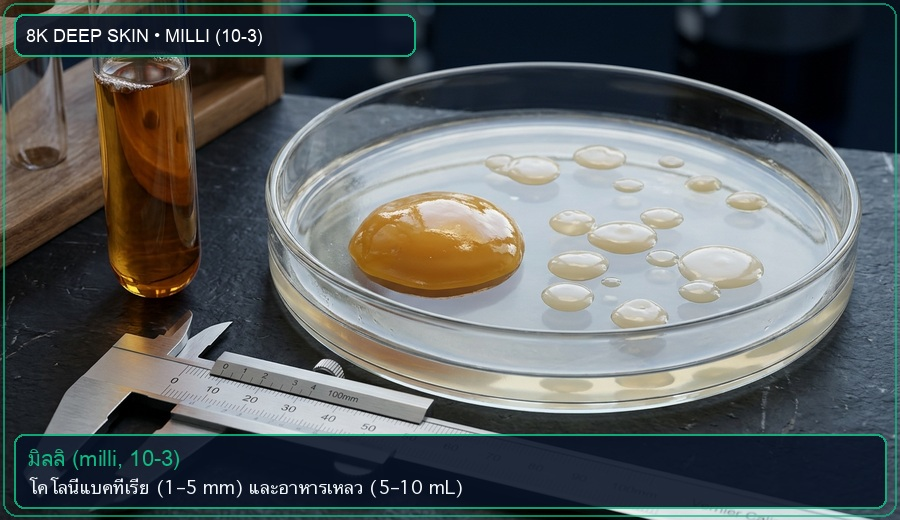
\includegraphics[width=3.65cm, height=2.05cm, keepaspectratio]{figures/sec_3d/prefix_milli.jpg}\vspace{1pt} \\
\midrule
ไมโคร\newline(micro) & $\mu$ & $10^{-6}$\newline$\left(\tfrac{1}{10^6}\right)$ &
\textbf{1. ระดับเซลล์ ($\mu\text{m}$)} วัดขนาดเซลล์แบคทีเรีย \textit{E. coli} ($1\text{--}2\text{ }\mu\text{m}$) และยีสต์กำลังแตกหน่อ ($5\text{--}10\text{ }\mu\text{m}$) ด้วยกล้องจุลทรรศน์ $1{,}000\times$\newline
\textbf{2. ปริมาตรไมโครปิเปต ($\mu\text{L}$)} ดูดสารละลายเชื้อและดีเอ็นเอด้วยไมโครปิเปต P20, P200, P1000 ($1\text{--}1{,}000\text{ }\mu\text{L}$) &
\vspace{1pt}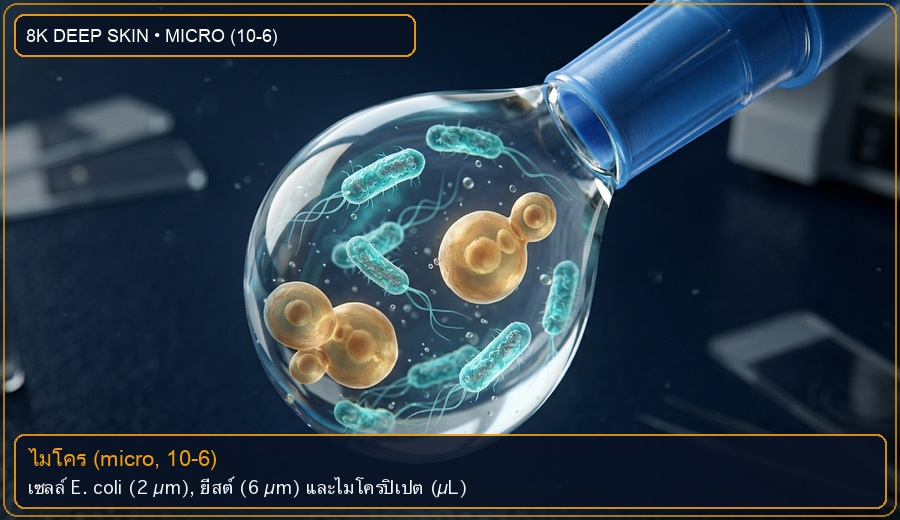
\includegraphics[width=3.65cm, height=2.05cm, keepaspectratio]{figures/sec_3d/prefix_micro.jpg}\vspace{1pt} \\
\midrule
นาโน\newline(nano) & $\text{n}$ & $10^{-9}$\newline$\left(\tfrac{1}{10^9}\right)$ &
\textbf{1. ระดับไวรัสและโมเลกุล ($\text{nm}$)} ระบุขนาดแบคทีริโอฟาจ T4 และไวรัส ($20\text{--}300\text{ nm}$) และรูพรุนแผ่นกรองปลอดเชื้อ ($220\text{ nm}$)\newline
\textbf{2. ความยาวคลื่นแสง ($\text{nm}$)} ตั้งค่าลำแสง $\lambda = 600\text{ nm}$ ($\text{OD}_{600}$) ในเครื่องสเปกโตรโฟโตมิเตอร์วัดความขุ่นของเซลล์ &
\vspace{1pt}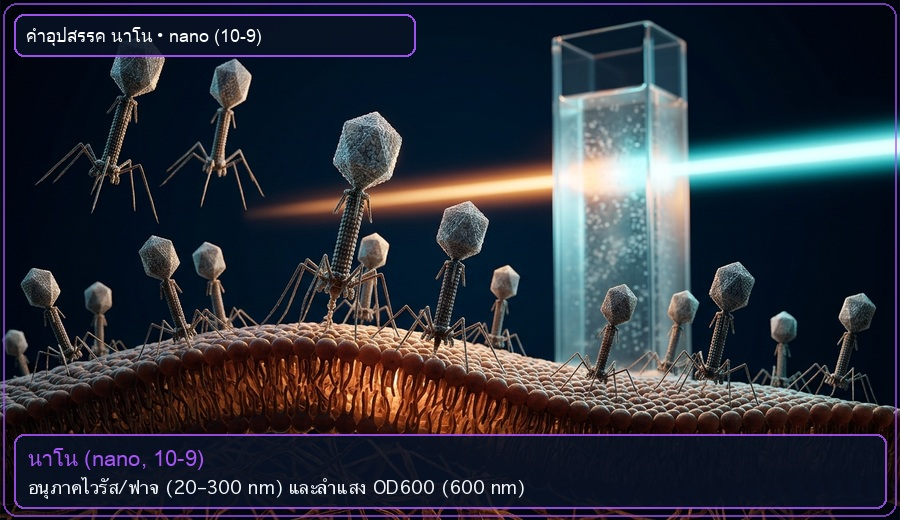
\includegraphics[width=3.65cm, height=2.05cm, keepaspectratio]{figures/sec_3d/prefix_nano.jpg}\vspace{1pt} \\
\bottomrule
\end{tabularx}
\end{table}

\section{การแปลงหน่วยโดยใช้เทคนิคบันไดเลื่อนจุดทศนิยม}

\deepskinfig{figures/sec_3d/ch01_s2.jpg}{บันไดคำอุปสรรคขั้นละ $1{,}000$ เท่า ($\text{m/L} \leftrightarrow \text{mm/mL} \leftrightarrow \mu\text{m/}\mu\text{L} \leftrightarrow \text{nm}$) สำหรับแปลงหน่วยขนาดเซลล์จุลินทรีย์และปริมาตรไมโครปิเปต}

นักศึกษาจำนวนมากมักสับสนเมื่อต้องคำนวณเลขยกกำลังติดลบ เช่น $10^{-6}$ หารด้วย $10^{-3}$ เพื่อขจัดปัญหานี้ เราสามารถใช้ \textbf{เทคนิคบันไดขั้นละ 1,000} (\textbf{Step-by-1,000 Ladder Method}) ซึ่งจำง่ายเหมือนการแลกธนบัตร กล่าวคือ หน่วยที่เรียงติดกันจากใหญ่ไปเล็ก ได้แก่ \textbf{หน่วยปกติ $\rightarrow$ มิลลิ ($\text{m}$) $\rightarrow$ ไมโคร ($\mu$) $\rightarrow$ นาโน ($\text{n}$)} จะมีค่าห่างกันขั้นละ $1{,}000$ เท่าเสมอ ดังแสดงใน\mbox{ภาพที่} 1.1

\begin{figure}[H]
\centering
\resizebox{0.88\textwidth}{!}{%
\begin{tikzpicture}[font=\sffamily, >=Stealth]
    % Steps
    \draw[fill=boxBlueBg, draw=physRoyalBlue, line width=1.4pt, rounded corners=3pt] (0,3.6) rectangle (3.6,4.6);
    \node[font=\bfseries\color{physRoyalBlue}] at (1.8,4.1) {หน่วยฐาน ($\text{m}, \text{L}, \text{g}$)};

    \draw[fill=boxGreenBg, draw=bioEmerald, line width=1.4pt, rounded corners=3pt] (3.8,2.4) rectangle (7.4,3.4);
    \node[font=\bfseries\color{bioEmerald!90!black}] at (5.6,2.9) {มิลลิ ($\text{mm}, \text{mL}, \text{mg}$)};

    \draw[fill=boxAmberBg, draw=physAmber, line width=1.4pt, rounded corners=3pt] (7.6,1.2) rectangle (11.2,2.2);
    \node[font=\bfseries\color{physAmber!90!black}] at (9.4,1.7) {ไมโคร ($\mu\text{m}, \mu\text{L}, \mu\text{g}$)};

    \draw[fill=boxPurpleBg, draw=labPurple, line width=1.4pt, rounded corners=3pt] (11.4,0.0) rectangle (15.0,1.0);
    \node[font=\bfseries\color{labPurple}] at (13.2,0.5) {นาโน ($\text{nm}, \text{ng}$)};

    % Arrows Down (Multiply by 1000)
    \draw[->, line width=1.5pt, color=crimsonAlert] (3.6,4.2) to[bend left=25] node[above right, font=\small\bfseries] {$\times 1{,}000$} (5.6,3.4);
    \draw[->, line width=1.5pt, color=crimsonAlert] (7.4,3.0) to[bend left=25] node[above right, font=\small\bfseries] {$\times 1{,}000$} (9.4,2.2);
    \draw[->, line width=1.5pt, color=crimsonAlert] (11.2,1.8) to[bend left=25] node[above right, font=\small\bfseries] {$\times 1{,}000$} (13.2,1.0);

    % Arrows Up (Divide by 1000)
    \draw[->, line width=1.5pt, color=physCyan] (3.8,2.6) to[bend left=25] node[below left, font=\small\bfseries] {$\div 1{,}000$} (1.8,3.6);
    \draw[->, line width=1.5pt, color=physCyan] (7.6,1.4) to[bend left=25] node[below left, font=\small\bfseries] {$\div 1{,}000$} (5.6,2.4);
    \draw[->, line width=1.5pt, color=physCyan] (11.4,0.2) to[bend left=25] node[below left, font=\small\bfseries] {$\div 1{,}000$} (9.4,1.2);
\end{tikzpicture}%
}
\caption{แผนภาพบันไดคำอุปสรรคขั้นละ 1,000 เท่า สำหรับการแปลงหน่วยขนาดเซลล์และปริมาตรสารละลาย}
\end{figure}

\vspace{4pt}
\arucomarkerbadge{0}{1}{ไมโครปิเปต P1000 และการเจือจางเชื้อแบบลำดับส่วน 3 มิติ}{จำลองกลไกลูกสูบไมโครปิเปต 2 จังหวะ และการดูดถ่ายสารละลายแบคทีเรียลดความเข้มข้นทีละ 10 เท่าพร้อมคำนวณค่า CFU/mL สด}{ปริมาตรดูด $V$ ($\mu\text{L}$), จำนวนขั้นการเจือจาง ($10^{-n}$), จำนวนโคโลนีบนจานเพาะเชื้อ}


\begin{conceptbox}[กฎทองของการแปลงหน่วยในห้องแล็บจุลชีววิทยา]
\begin{itemize}
    \item \textbf{แปลงจากหน่วยใหญ่ไปหน่วยเล็ก} (เดินลงบันได 1 ขั้น)\quad \textbf{ให้คูณด้วย $1{,}000$} (หรือเลื่อนจุดทศนิยมไปทางขวา 3 ตำแหน่ง) เช่น $1\text{ mL} = 1{,}000\text{ }\mu\text{L}$ และ $1\text{ }\mu\text{m} = 1{,}000\text{ nm}$
    \item \textbf{แปลงจากหน่วยเล็กไปหน่วยใหญ่} (เดินขึ้นบันได 1 ขั้น)\quad \textbf{ให้หารด้วย $1{,}000$} (หรือเลื่อนจุดทศนิยมไปทางซ้าย 3 ตำแหน่ง) เช่น $250\text{ }\mu\text{L} = 0.250\text{ mL}$
\end{itemize}
\end{conceptbox}

\begin{worked}[การแปลงหน่วยขนาดเซลล์แบคทีเรียและปริมาตรไมโครปิเปต]
\textbf{โจทย์ปัญหา}\quad นักศึกษาจุลชีววิทยาส่องกล้องจุลทรรศน์พบเซลล์แบคทีเรีย \textit{Bacillus subtilis} มีความยาวเฉลี่ย $4.5\text{ }\mu\text{m}$ และในการเตรียมปฏิกิริยาพีซีอาร์ (PCR) ต้องใช้ไมโครปิเปตดูดสารละลายบัฟเฟอร์ปริมาตร $0.05\text{ mL}$ จงหาว่า (ก) แบคทีเรียชนิดนี้มีความยาวกี่มิลลิเมตร ($\text{mm}$) และกี่นาโนเมตร ($\text{nm}$) และ (ข) ต้องตั้งค่าไมโครปิเปตเป็นกี่ไมโครลิตร ($\mu\text{L}$)

\textbf{วิธีทำทีละขั้นตอนฉบับเข้าใจง่าย}
\begin{enumerate}
    \item \textbf{ขั้นที่ 1 แปลงความยาวแบคทีเรีย $4.5\text{ }\mu\text{m}$ เป็น $\text{mm}$ และ $\text{nm}$}
    \begin{itemize}
        \item จาก $\mu\text{m}$ ไปเป็น $\text{mm}$ คือการเดินขึ้นบันได 1 ขั้น (หน่วยเล็กไปหน่วยใหญ่) จึงนำมา\textbf{หารด้วย $1{,}000$}
        \[
            \text{ความยาวในหน่วยมิลลิเมตร} = \frac{4.5}{1{,}000} = 0.0045\text{ mm}
        \]
        \item จาก $\mu\text{m}$ ไปเป็น $\text{nm}$ คือการเดินลงบันได 1 ขั้น (หน่วยใหญ่ไปหน่วยเล็ก) จึงนำมา\textbf{คูณด้วย $1{,}000$}
        \[
            L_{\text{nm}} = 4.5 \times 1{,}000 = 4{,}500\text{ nm}
        \]
    \end{itemize}
    \item \textbf{ขั้นที่ 2 แปลงปริมาตรสารละลาย $0.05\text{ mL}$ เป็น $\mu\text{L}$}
    \begin{itemize}
        \item จาก $\text{mL}$ ไปเป็น $\mu\text{L}$ คือการเดินลงบันได 1 ขั้น จึงนำมา\textbf{คูณด้วย $1{,}000$}
        \[
            \text{ปริมาตรไมโครปิเปต} = 0.05 \times 1{,}000 = 50\text{ }\mu\text{L}
        \]
    \end{itemize}
\end{enumerate}
\textbf{คำตอบ}\quad แบคทีเรียมีความยาวเท่ากับ $0.0045\text{ mm}$ หรือ $4{,}500\text{ nm}$ และต้องตั้งค่าไมโครปิเปตที่ $50\text{ }\mu\text{L}$
\end{worked}

\section{เลขนัยสำคัญ ความเที่ยง ความแม่น และความคลาดเคลื่อนของการวัด}

\deepskinfig{figures/sec_3d/ch01_s3.jpg}{กลไกปุ่มกด 2 จังหวะของไมโครปิเปต P1000 และการตรวจสอบความแม่น (Accuracy) ด้วยการชั่งมวลน้ำกลั่นบนเครื่องชั่งดิจิทัลละเอียดทศนิยม 4 ตำแหน่ง}

ในการบันทึกผลการทดลองทางวิทยาศาสตร์ ตัวเลขทุกตัวที่เขียนลงในตารางบันทึกผลต้องสะท้อนความละเอียดของเครื่องมือวัดจริง ซึ่งเรียกว่า \textbf{เลขนัยสำคัญ} (\textbf{Significant Figures}) โดยประกอบด้วยตัวเลขที่อ่านได้แน่นอนจากขีดสเกลรวมกับตัวเลขประมาณค่าอีก 1 ตำแหน่ง นอกจากนี้ นักจุลชีววิทยาต้องแยกแยะความแตกต่างระหว่าง \textbf{ความแม่น} (\textbf{Accuracy} คือความใกล้เคียงกับค่าจริงมาตรฐาน) และ \textbf{ความเที่ยง} (\textbf{Precision} คือความสม่ำเสมอหรือการซ้ำรอยเดิมเมื่อวัดซ้ำหลายครั้ง)

หากเราต้องการตรวจสอบว่าไมโครปิเปตในห้องปฏิบัติการยังมีความแม่นยำหรือไม่ เราสามารถใช้วิธีชั่งมวลของน้ำกลั่นที่ดูดออกมา เนื่องจากน้ำบริสุทธิ์ที่อุณหภูมิห้องมีความหนาแน่นประมาณ $1\text{ g/mL}$ หรือกล่าวได้ว่า \textbf{น้ำกลั่นปริมาตร $1{,}000\text{ }\mu\text{L}$ ($1\text{ mL}$) จะมีมวลเท่ากับ $1.0000\text{ g}$ และน้ำกลั่น $100\text{ }\mu\text{L}$ จะมีมวลเท่ากับ $0.1000\text{ g}$} โดยคำนวณเปอร์เซ็นต์ความคลาดเคลื่อนสัมพัทธ์ได้จากสมการที่ (1.1)

\begin{equation}
    \text{เปอร์เซ็นต์ความคลาดเคลื่อน} = \frac{|\text{ค่าที่วัดได้จริง} - \text{ค่ามาตรฐาน}|}{\text{ค่ามาตรฐาน}} \times 100\%
\end{equation}

\begin{warningbox}[ห้ามกดปุ่มไมโครปิเปตเลยจังหวะแรกขณะดูดสารละลาย]
ไมโครปิเปตมีปุ่มกด 2 จังหวะ (\textbf{First Stop} และ \textbf{Second Stop}) ขณะจุ่มปลายทิปเพื่อดูดสารละลายหรือเชื้อจุลินทรีย์ \textbf{ต้องกดลงไปเพียงจังหวะแรกเท่านั้น} แล้วค่อยๆ ผ่อนนิ้วขึ้น หากเผลอกดลงไปถึงจังหวะที่สองขณะดูดสาร จะทำให้ได้ปริมาตรเกินกว่าที่ตั้งไว้ถึง 10--15\% ส่วนจังหวะที่สองมีไว้ใช้ตอนปล่อยสารออกจากปลายทิปให้หมดจดเท่านั้น
\end{warningbox}

\section{ปฏิบัติการประจำสัปดาห์ที่ 1}

\deepskinfig{figures/sec_3d/ch01_s4.jpg}{ชุดอุปกรณ์ปฏิบัติการที่ 1 ประกอบด้วยเวอร์เนียร์คาลิปเปอร์วัดขนาดจานเพาะเชื้อ ไมโครมิเตอร์วัดความหนาสไลด์แก้ว และไมโครปิเปต P1000 พร้อมเครื่องชั่งดิจิทัล}

\begin{labbox}[ปฏิบัติการที่ 1\quad การวัดละเอียดและทักษะการใช้ไมโครปิเปตและเครื่องชั่งดิจิทัล (3 ชั่วโมง)]
\noindent\textbf{ผลลัพธ์การเรียนรู้ที่ประเมิน}\quad CLO1 (ความรู้การวัดและแปลงหน่วย), CLO3 (วินัย ความปลอดภัย และความซื่อสัตย์ในการบันทึกข้อมูลจริง), CLO4 (การทำงานร่วมกันและเขียนรายงาน)

\vspace{4pt}
\noindent\textbf{1. วัสดุและอุปกรณ์}
\begin{itemize}
    \item เวอร์เนียร์คาลิปเปอร์ (ความละเอียด $0.05\text{ mm}$) และไมโครมิเตอร์ (ความละเอียด $0.01\text{ mm}$)
    \item จานเพาะเชื้อแก้ว (Petri Dish), หลอดทดลอง (Test Tube) และแผ่นสไลด์กล้องจุลทรรศน์
    \item ไมโครปิเปตขนาด P1000 ($100\text{--}1{,}000\text{ }\mu\text{L}$) และ P200 ($20\text{--}200\text{ }\mu\text{L}$) พร้อมทิปปลอดเชื้อ
    \item เครื่องชั่งดิจิทัลละเอียดทศนิยม 4 ตำแหน่ง บีกเกอร์ใส่น้ำกลั่น และผงวุ้นอาหารเลี้ยงเชื้อจำลอง (โซเดียมคลอไรด์)
\end{itemize}

\noindent\textbf{2. ขั้นตอนการทดลอง}
\begin{enumerate}
    \item \textbf{ตอนที่ 1 การวัดมิติภาชนะทางจุลชีววิทยา}\quad ใช้เวอร์เนียร์คาลิปเปอร์วัดเส้นผ่านศูนย์กลางภายในและความลึกของจานเพาะเชื้อจำนวน 3 ครั้ง และใช้ไมโครมิเตอร์วัดความหนาของแผ่นสไลด์แก้วจำนวน 3 ครั้ง บันทึกค่าเฉลี่ยและแปลงหน่วยเป็นไมโครเมตร ($\mu\text{m}$)
    \item \textbf{ตอนที่ 2 การตรวจสอบความแม่นและความเที่ยงของไมโครปิเปต}\quad วางบีกเกอร์พลาสติกขนาดเล็กบนเครื่องชั่งดิจิทัลแล้วกดปุ่มเซตศูนย์ (\textbf{Tare}) จากนั้นตั้งค่าไมโครปิเปต P1000 ที่ปริมาตร $500\text{ }\mu\text{L}$ ดูดน้ำกลั่นหยดลงในบีกเกอร์ อ่านค่ามวลเป็นกรัม ($\text{g}$) ทำซ้ำ 3 ครั้ง แล้วคำนวณค่าเฉลี่ยและเปอร์เซ็นต์ความคลาดเคลื่อนเทียบกับค่ามาตรฐาน $0.5000\text{ g}$
\end{enumerate}

\noindent\textbf{3. ตารางบันทึกผลการทดลอง (สำหรับนักศึกษาบันทึกค่าจริงในห้องปฏิบัติการ)}
\begin{center}
\footnotesize\setlength{\tabcolsep}{3.5pt}
\begin{tabularx}{\linewidth}{>{\raggedright\arraybackslash}X c c c c c}
\toprule
\textbf{รายการที่วัด} & \textbf{ครั้งที่ 1} & \textbf{ครั้งที่ 2} & \textbf{ครั้งที่ 3} & \textbf{ค่าเฉลี่ย} & \textbf{หน่วย $\mu\text{m}$ / $\mu\text{L}$} \\
\midrule
เส้นผ่านศูนย์กลางจานเพาะเชื้อ ($\text{mm}$) & ............ & ............ & ............ & ............ & \dotfill $\mu\text{m}$ \\
ความหนาของแผ่นสไลด์แก้ว ($\text{mm}$) & ............ & ............ & ............ & ............ & \dotfill $\mu\text{m}$ \\
มวลน้ำกลั่นจากปิเปต $500\text{ }\mu\text{L}$ ($\text{g}$) & ............ & ............ & ............ & ............ & คลาดเคลื่อน ............ \% \\
\bottomrule
\end{tabularx}
\end{center}
\end{labbox}

\section*{คำถามท้ายบทที่ 1 (ทบทวนแนวคิดและการคำนวณเบื้องต้น)}
\begin{enumerate}
    \item เซลล์ยีสต์ \textit{Saccharomyces cerevisiae} มีเส้นผ่านศูนย์กลางประมาณ $6\text{ }\mu\text{m}$ จงแปลงค่าดังกล่าวให้เป็นหน่วยมิลลิเมตร ($\text{mm}$) และนาโนเมตร ($\text{nm}$) โดยใช้เทคนิคบันไดขั้นละ $1{,}000$
    \item หากต้องการเตรียมสารละลายยาปฏิชีวนะปริมาตร $0.25\text{ mL}$ นักศึกษาควรเลือกใช้ไมโครปิเปตขนาดใดระหว่าง P20, P200 หรือ P1000 และต้องตั้งตัวเลขเป็นกี่ไมโครลิตร ($\mu\text{L}$) เพราะเหตุใด
    \item ในการทดสอบไมโครปิเปตที่ตั้งค่าไว้ $200\text{ }\mu\text{L}$ นักศึกษาชั่งมวลน้ำกลั่น 3 ครั้ง ได้ค่า $0.198\text{ g}$, $0.199\text{ g}$ และ $0.197\text{ g}$ จงหาค่าเฉลี่ยและเปอร์เซ็นต์ความคลาดเคลื่อนเทียบกับค่ามาตรฐาน $0.200\text{ g}$
\end{enumerate}
